
\documentclass{article}
\usepackage[T1]{fontenc}
\usepackage{graphicx}
\usepackage{amsmath, amsthm, amssymb}
\usepackage{hyperref}
\usepackage{polski}
\usepackage{listings}
\usepackage{color}
\usepackage{enumerate}
\usepackage{float}
\usepackage{longtable}
\lstset{
	language=C++,
	basicstyle=\ttfamily\footnotesize,
	keywordstyle=\color{blue}\bfseries,
	commentstyle=\color{green},
	stringstyle=\color{red},
	numberstyle=\tiny\color{green},
	numbers=left,
	stepnumber=1,
	tabsize=4,
	breaklines=true,
	showstringspaces=false
}
\title{Raport AiSD lista 2}
\author{Amelia Dorożko}
\date{\today}

\begin{document}
\section{Sortowanie szybkie}
\subsection{\texttt{QUICK\_SORT}}
Algorytm \texttt{QUICK\_SORT} polega na wyborze elementu zwanego pivotem, który  jest ostatnim elementem tablicy. Następnie za pomocą \texttt{PARITION} dzieli tablicę na dwie części: elementy mniejsze od pivota znajdują się po jego lewej stronie, a większe po prawej. Po podziale  rekurencyjnie sortuje obie podtablice. Średnia złożoność czasowa tego algorytmu wynosi \(O(n \log n)\). Jednak w najgorszym przypadku, gdy podział jest bardzo nierówny (np. dla tablicy posortowanej), czas działania wzrasta do \(O(n^2)\).

\subsection{\texttt{QUICK\_SORT}-z dwoma pivotami}


\texttt{QUICK\_SORT2} to modyfikacja, która wykorzystuje dwa pivoty zamiast jednego. Tablica dzielona jest na trzy części: elementy mniejsze od pierwszego pivota, elementy pomiędzy dwoma pivotami oraz elementy większe od drugiego pivota. Podczas \texttt{PARTITION2} algorytm najpierw porównuje oba pivoty i w razie potrzeby zamienia je miejscami, aby pierwszy pivot był mniejszy od drugiego. Następnie elementy są przypisywane do odpowiednich części: na początek (mniejsze niż pierwszy pivot), na koniec (większe niż drugi pivot) lub pozostają między pivotami. Po partycjonowaniu algorytm rekurencyjnie sortuje każdą z trzech części tablicy.

	\begin{table}[h]
		\centering
		\caption{Liczba porównań i przypisań dla \texttt{QUICK\_SORT} i \texttt{QUICK\_SORT2}} dla liczb z zakresu [-100,100]
		\label{tab:qs_classic}
		\begin{tabular}{|c|c|c|c|c|}
			\hline
			\textbf{Długość tablicy} & \textbf{QS:porównania} & \textbf{QS: przypisania} & \textbf{QS2: porównania} & \textbf{QS2: przypisania} \\ \hline
			10                      & 38                          & 36                          & 39                           & 58                           \\ \hline
			100                     & 802                         & 744                         & 530                          & 682                          \\ \hline
			200                     & 1725                        & 1794                        & 1149                         & 1558                         \\ \hline
			400                     & 4002                        & 3762                        & 2659                         & 3264                         \\ \hline
			600                     & 6621                        & 6866                        & 4088                         & 5424                         \\ \hline
			800                     & 9262                        & 9674                        & 6325                         & 8524                         \\ \hline
			1000                    & 11873                       & 11104                       & 7942                         & 11026                        \\ \hline
		\end{tabular}
	\end{table}


Wykorzystanie dwóch pivotów zmniejsza liczbę poziomów rekurencji. Dzięki temu algorytm staje się bardziej wydajny pod względem liczby porównań i przypisań, szczególnie w przypadku dużych, zróżnicowanych zbiorów danych. Wprowadzenie podwójnego pivota optymalizuje proces sortowania i zmniejsza ryzyko degeneracji algorytmu, co czyni go bardziej wszechstronnym w praktyce.

\section{Sortowanie przez zliczanie i sortowanie pozycyjne}
\subsection{\texttt{COUNTING\_SORT}}
Algorytm ten wykorzystuje tablicę pomocniczą do zliczania wystąpień poszczególnych elementów w zbiorze danych. Jest to algorytm stabilny i działa w czasie liniowym  \emph{O($n$)}.
Dla każdego elementu w tablicy \( A \) obliczana jest cyfra na określonej pozycji. Cyfra ta jest obliczana przy użyciu wyrażenia:
\[
\left( \frac{A[i]}{k} \right) \% d
\]
gdzie:
\begin{itemize}
	\item \( k \) to miejsce,
	\item \( d \) to liczba cyfr (w systemie dziesiętnym jest to 10),
	\item \( A[i] \) to element tablicy \( A \).
\end{itemize}
Wartości cyfr są zliczane w tablicy pomocniczej \( C \).
\subsection{\texttt{RADIX\_SORT}}
\texttt{RADIX\_SORT} to algorytm sortowania oparty na metodzie sortowania pozycyjnego. Zamiast porównywać liczby bezpośrednio, sortuje dane w kolejnych krokach, zaczynając od najmniej znaczącej cyfry (cyfrach jedności), a kończąc na najbardziej znaczącej cyfrze.Używa \texttt{COUNTING\_SORT} do sortowania cyfr na kolejnych miejscach w liczbach
\subsection{\texttt{RADIX\_SORT}-dla liczb ujemnych}
Ta modyfikacja algorytmu Radix Sort umożliwia sortowanie liczb zarówno dodatnich, jak i ujemnych. Przed rozpoczęciem sortowania, dane są dzielone na liczby dodatnie i ujemne. Liczby ujemne są przechowywane w osobnej tablicy, a następnie przekształcone na liczby dodatnie. Następnie, takie dwie tablice są sortowane przy użyciu klasycznego \texttt{RADIX\_SORT}.
\begin{lstlisting}

void RADIX_SORT_WITH_NEGATIVES(int A[], int n, int d) {
	int negative_count = 0, positive_count = 0;
	for (int i = 0; i <= n; i++){
		if (A[i]<0){
			negative_count++;
			liczbaPorownan++;
		}
		if (A[i]>0){
			positive_count++;
			liczbaPorownan++;
		}
	}
	int negatives[negative_count], positives[positive_count];
	int neg_index = 0, pos_index = 0;
	
	for (int i = 0; i < n; i++) {
		if (A[i] < 0) {
			negatives[neg_index++] = -A[i];
			liczbaPrzypisan++;
		} else {
			positives[pos_index++] = A[i];
			liczbaPrzypisan++;
		}
		liczbaPorownan++;
	}
\end{lstlisting}
Podstawa \(d\) wpływa również na rozmiar bucketów, do których będą trafiały elementy w trakcie sortowania. Zwiększenie liczby grup (w przypadku większej podstawy \(d\)) może pomóc w szybszym rozdzieleniu elementów, ale z drugiej strony wiąże się z większymi wymaganiami pamięciowymi. Zmiana podstawy może wpłynąć na efektywność przestrzenną i czasową algorytmu. Większa podstawa może zmniejszyć liczbę iteracji. Idzie zauważyć, że wzrost ten jest liniowy.


\begin{figure}[H]
	\centering
	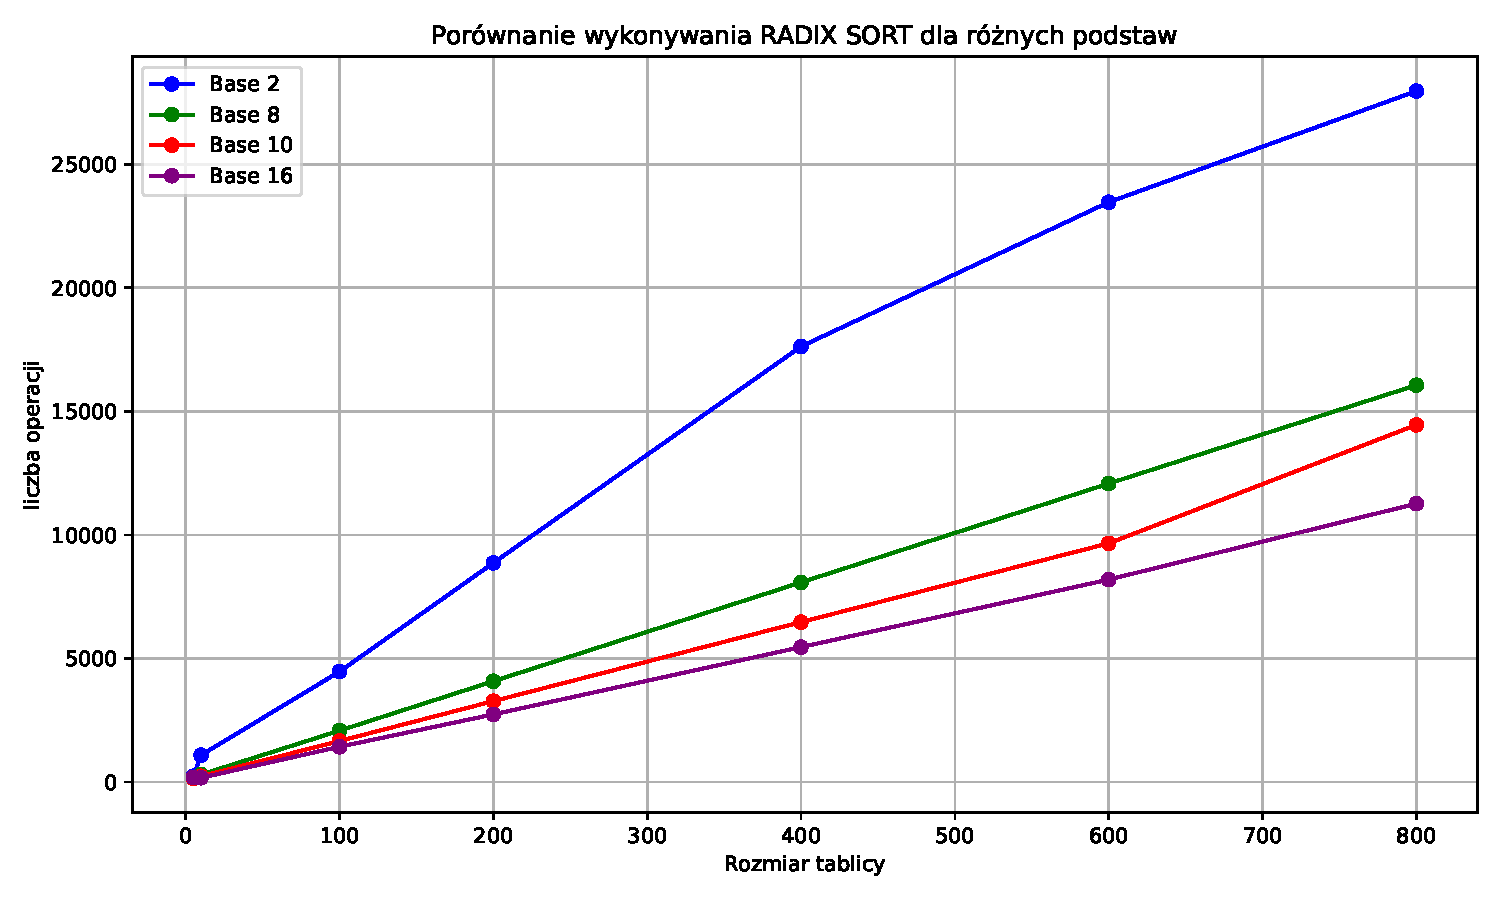
\includegraphics[width=1\textwidth]{wykres2.pdf}
\end{figure}


	\begin{table}[H]
	\centering
	\begin{tabular}{|c|c|c|c|c|}
		\hline
		\textbf{Długość tablicy} & \textbf{Podstawa 2} & \textbf{Podstawa 8} & \textbf{Podstawa 10} & \textbf{Podstawa 16} \\
		\hline
		5   & Porównania: 12  & Porównania: 13  & Porównania: 13  & Porównania: 13  \\
		& Przypisania: 220 & Przypisania: 144 & Przypisania: 137 & Przypisania: 173 \\
		\hline
		10  & Porównania: 23  & Porównania: 23  & Porównania: 23  & Porównania: 18  \\
		& Przypisania: 1061 & Przypisania: 276 & Przypisania: 207 & Przypisania: 151 \\
		\hline
		100 & Porównania: 203 & Porównania: 203 & Porównania: 202 & Porównania: 202 \\
		& Przypisania: 4261 & Przypisania: 1873 & Przypisania: 1454 & Przypisania: 1221 \\
		\hline
		200 & Porównania: 403 & Porównania: 403 & Porównania: 403 & Porównania: 402 \\
		& Przypisania: 8461 & Przypisania: 3673 & Przypisania: 2867 & Przypisania: 2331 \\
		\hline
		400 & Porównania: 802 & Porównania: 803 & Porównania: 803 & Porównania: 803 \\
		& Przypisania: 16820 & Przypisania: 7273 & Przypisania: 5667 & Przypisania: 4654 \\
		\hline
		600 & Porównania: 1203 & Porównania: 1203 & Porównania: 1202 & Porównania: 1202 \\
		& Przypisania: 22261 & Przypisania: 10873 & Przypisania: 8454 & Przypisania: 6987 \\
		\hline
		800 & Porównania: 1603 & Porównania: 1602 & Porównania: 1603 & Porównania: 1602 \\
		& Przypisania: 33661 & Przypisania: 23851 & Przypisania: 12848 & Przypisania: 9662 \\
		\hline
	\end{tabular}
	\caption{Porównanie wyników dla różnych podstaw w Radix Sort z danymi dodatnimi i ujemnymi}
	
\end{table}

\section{Sortowanie kubełkowe}
\subsection{\texttt{BUCKET\_SORT}}
Algorytm \texttt{BUCKET\_SORT} jest sortowaniem rozdzielającym, które polega na podzieleniu danych wejściowych na "kubełki", a następnie sortowaniu ich indywidualnie za pomocą innego algorytmu sortowania (zwykle \texttt{INSERTION\_SORT}). Po posortowaniu elementów w kubełkach, wyniki są scalane z powrotem w jedną posortowaną tablicę.\\
Pierwsza wersja algorytmu zakłada, że dane wejściowe są liczbami zmiennoprzecinkowymi mniejszymi od 1 i większymi, bądź równymi zero.


\subsubsection{\texttt{BUCKET\_SORT} dla dowolnych liczb}
Druga wersja algorytmu została zmodyfikowana, aby działała dla liczb \textbf{dowolnego przedziału}. Zakłada się, że dane mogą pochodzić z dowolnego przedziału liczbowego.

\begin{itemize}
	\item \textbf{Znalezienie min i max:} Pierwszym krokiem jest znalezienie minimalnej (\texttt{minValue}) i maksymalnej (\texttt{maxValue}) wartości w tablicy. Dzięki temu możemy obliczyć zakres danych.
	
	\item \textbf{Przypisanie do kubełków:} Następnie dane są rozdzielane na kubełki w sposób, który uwzględnia minimalną i maksymalną wartość. 

	gdzie \(\text{range}\) to różnica między największą a najmniejszą wartością w tablicy. Dzięki temu każdemu elementowi przypisywana jest odpowiednia pozycja w jednym z kubełków.
	
\begin{lstlisting}
	
	
	void BUCKET_SORT2(double A[], int n) {
		double minValue = A[0];
		double maxValue = A[0];

		for (int i = 1; i < n; i++) {
			if (A[i] < minValue) {
				minValue = A[i];
			}
			
			if (A[i] > maxValue) {
				maxValue = A[i];
			}
		}
		
		double range = maxValue - minValue;
		List B[n];
		for (int j = 0; j < n; j++) {
			B[j] = List();

		}
		
		for (int i = 0; i < n; ++i) {
			int bucketIndex = static_cast<int>(((A[i] - minValue) / range) * n);
			if (bucketIndex == n) bucketIndex--;
			LIST_INSERT(B[bucketIndex], new Node(A[i]));
\end{lstlisting}
\item Dalej kod działa tak jak dla "normalnego" \texttt{BUCKET\_SORT}, czyli sortujemy liczby w kubełkach używając \texttt{INSERTION\_SORT}, a następnie scalając.
	
\end{itemize}

\subsection{Złożoność algorytmu}
Złożoność czasowa algorytmu zależy od kilku czynników, takich jak liczba kubełków, liczba elementów w tablicy oraz wybrany algorytm do sortowania danych w kubełkach. Złożoność dla \texttt{BUCKET\_SORT} w najlepszym przypadku wynosi \(O(n)\), ale w najgorszym przypadku może osiągnąć \(O(n^2)\), szczególnie gdy dane są nierównomiernie rozłożone w kubełkach. 
	
\section{\texttt{INSERTION\_SORT} na listach}
Warto zwrócić uwagę, że algorytm wykorzystany przez \texttt{BUCKET\_SORT}, który używany jest do posortowania elementów wewnątrz poszczególnych bucketów. W kontekście implementacji na listach dwukierunkowych, \texttt{INSERTION\_SORT} operuje bezpośrednio na węzłach, co pozwala na sprawne zarządzanie strukturą listy.Jest on skuteczny dla małych zbiorów danych, w szczególności w kubełkach. 
	
\subsection{Porównanie wydajności algorytmów}
\texttt{QUCIK\_SORT} jest bardziej wszechstronny, natomiast \texttt{BUCKET\_SORT} działa najlepiej, gdy dane są równomiernie rozłożone w małym zakresie.

\begin{figure}[H]
	\centering
	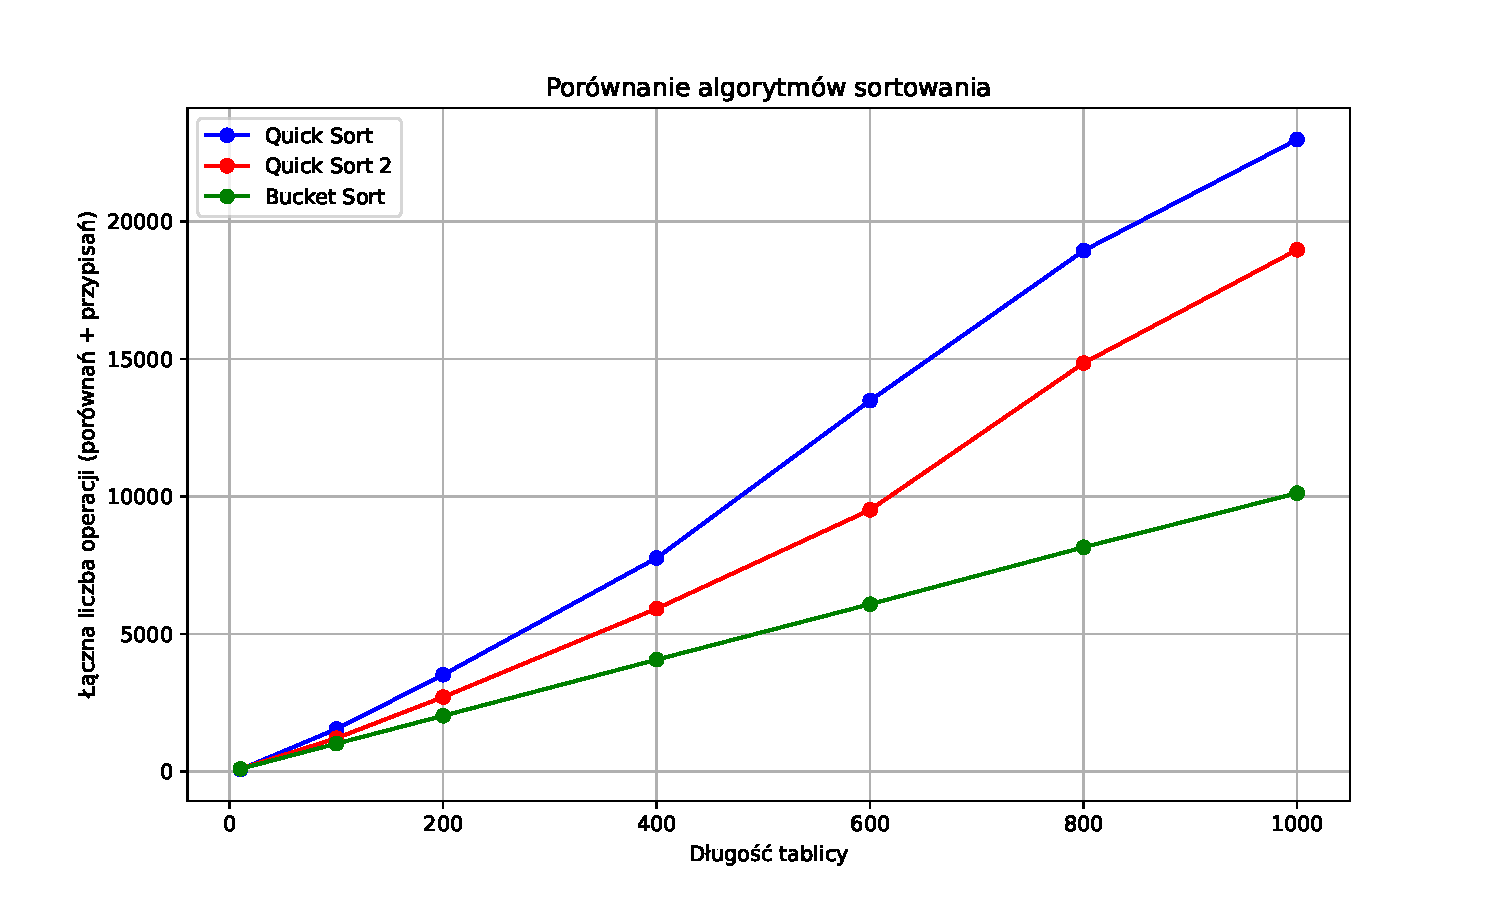
\includegraphics[width=1\textwidth]{wykres1.pdf}
\end{figure}
 Tutaj porównujemy działanie algorytmów dla liczb z przedziału [0,1):
 
 \begin{figure}[H]
 	\centering
 	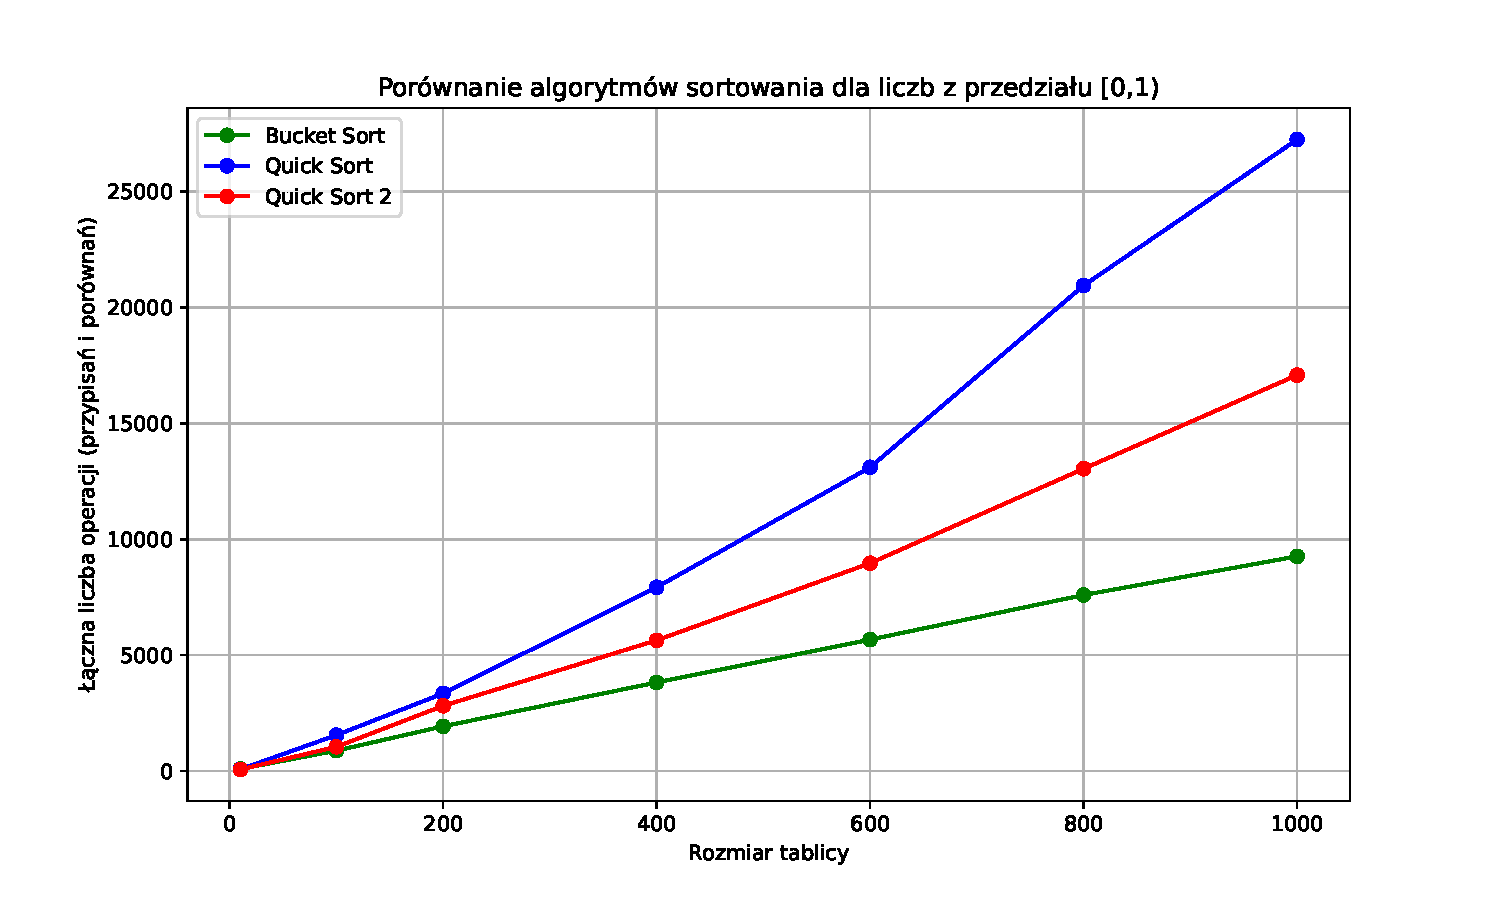
\includegraphics[width=1\textwidth]{wykres.3.pdf}
 \end{figure}
 Jak widać różnica w działaniu tych algorytmów jest niewielka, najbardziej efektywnym algorytmem pozostaje \texttt{BUCKET\_SORT}. 

	
	
\end{document}